% Preamble templated from Dhawal24112006/EE1030
\documentclass{beamer}
\mode<presentation>
\usepackage{amsmath}
\usepackage{amssymb}
% \usepackage{advdate}
\usepackage{adjustbox}
\usepackage{subcaption}
% \usepackage{enumitem}
\usepackage{multicol}
\usepackage{mathtools}
\usepackage{listings}
\usepackage{url}
% \def\UrlBreaks{\do\/\do-}
\usetheme{Boadilla}
\usecolortheme{lily}
\setbeamertemplate{footline}
{
  \leavevmode%
  \hbox{%
  \begin{beamercolorbox}[wd=\paperwidth,ht=2.25ex,dp=1ex,right]{author in head/foot}%
    \insertframenumber{} / \inserttotalframenumber\hspace*{2ex}
  \end{beamercolorbox}}%
  \vskip0pt%
}
\setbeamertemplate{navigation symbols}{}

\providecommand{\nCr}[2]{\,^{#1}C_{#2}} % nCr
\providecommand{\nPr}[2]{\,^{#1}P_{#2}} % nPr
\providecommand{\mbf}{\mathbf}
\providecommand{\pr}[1]{\ensuremath{\Pr\left(#1\right)}}
\providecommand{\qfunc}[1]{\ensuremath{Q\left(#1\right)}}
\providecommand{\sbrak}[1]{\ensuremath{{}\left[#1\right]}}
\providecommand{\lsbrak}[1]{\ensuremath{{}\left[#1\right.}}
\providecommand{\rsbrak}[1]{\ensuremath{{}\left.#1\right]}}
\providecommand{\brak}[1]{\ensuremath{\left(#1\right)}}
\providecommand{\lbrak}[1]{\ensuremath{\left(#1\right.}}
\providecommand{\rbrak}[1]{\ensuremath{\left.#1\right)}}
\providecommand{\cbrak}[1]{\ensuremath{\left\{#1\right\}}}
\providecommand{\lcbrak}[1]{\ensuremath{\left\{#1\right.}}
\providecommand{\rcbrak}[1]{\ensuremath{\left.#1\right\}}}
\theoremstyle{remark}
\newtheorem{rem}{Remark}
\newcommand{\sgn}{\mathop{\mathrm{sgn}}}
\providecommand{\abs}[1]{\left\vert#1\right\vert}
\providecommand{\res}[1]{\Res\displaylimits_{#1}}
\providecommand{\norm}[1]{\lVert#1\rVert}
\providecommand{\mtx}[1]{\mathbf{#1}}
\providecommand{\mean}[1]{E\left[ #1 \right]}
\providecommand{\fourier}{\overset{\mathcal{F}}{ \rightleftharpoons}}
%\providecommand{\hilbert}{\overset{\mathcal{H}}{ \rightleftharpoons}}
\providecommand{\system}{\overset{\mathcal{H}}{ \longleftrightarrow}}
%\newcommand{\solution}[2]{\textbf{Solution:}{#1}}
%\newcommand{\solution}{\noindent \textbf{Solution: }}
\providecommand{\dec}[2]{\ensuremath{\overset{#1}{\underset{#2}{\gtrless}}}}
\newcommand{\myvec}[1]{\ensuremath{\begin{pmatrix}#1\end{pmatrix}}}
\let\vec\mathbf

\lstset{
% %language=C,
frame=single,
breaklines=true,
columns=fullflexible,
showstringspaces=false
}

\numberwithin{equation}{section}

\title{MATGEO Presentation: 4.7.52}
\author{Subhodeep Chakraborty \\ ee25btech11055,\\IIT Hyderabad.}

\date{\today}
\begin{document}

\begin{frame}
\titlepage
\end{frame}

\section*{Outline}
\begin{frame}
\tableofcontents
\end{frame}

\section{Problem}
\begin{frame}
\frametitle{Problem Statement}

If the points \brak{1, 1, p} and \brak{-3, 0, 1} be equidistant from the plane $\vec{r}\cdot\brak{3\hat{\imath} + 4\hat{\jmath} -12\hat{k}}+13=0$, then find the value of $p$.

\end{frame}

\section{Solution}
\begin{frame}{Given data points}
Given:
\begin{align}
 \vec{A} = \myvec{1 \\ 1 \\ p} \\
 \vec{B} = \myvec{-3 \\ 0 \\1 } \\
 \vec{S}: \myvec{3 & 4 & -12}\cdot\vec{r} = -13
\end{align}
\end{frame}

\begin{frame}{Formulae}
We know distance of point $\vec{P}$ from plane $\vec{n}^\top\vec{x}=c$ is given by:
\begin{align}
 d = \frac{|\vec{n}^\top\vec{P}-c|}{\norm{\vec{n}}}
\end{align}
\end{frame}

\begin{frame}{Solving}
Thus
\begin{align}
 \frac{|\vec{n}^\top\vec{A}-c|}{\norm{\vec{n}}} &= \frac{|\vec{n}^\top\vec{B}-c|}{\norm{\vec{n}}} \\
 \vec{n}^\top\vec{A} = \vec{n}^\top\vec{B} &\text{ OR } \vec{n}^\top\vec{A} = 2c - \vec{n}^\top\vec{B}
\end{align}
Substituting values
\begin{align}
7 - 12p = -21 &\textbf{  OR  } 7-12p = -26 + 21 \\
p = 7/3 &\textbf{  OR  } p = 1
\end{align}
\end{frame}

\subsection{Plot}
\begin{frame}{Plot}
 \begin{figure}[H]
    \centering
    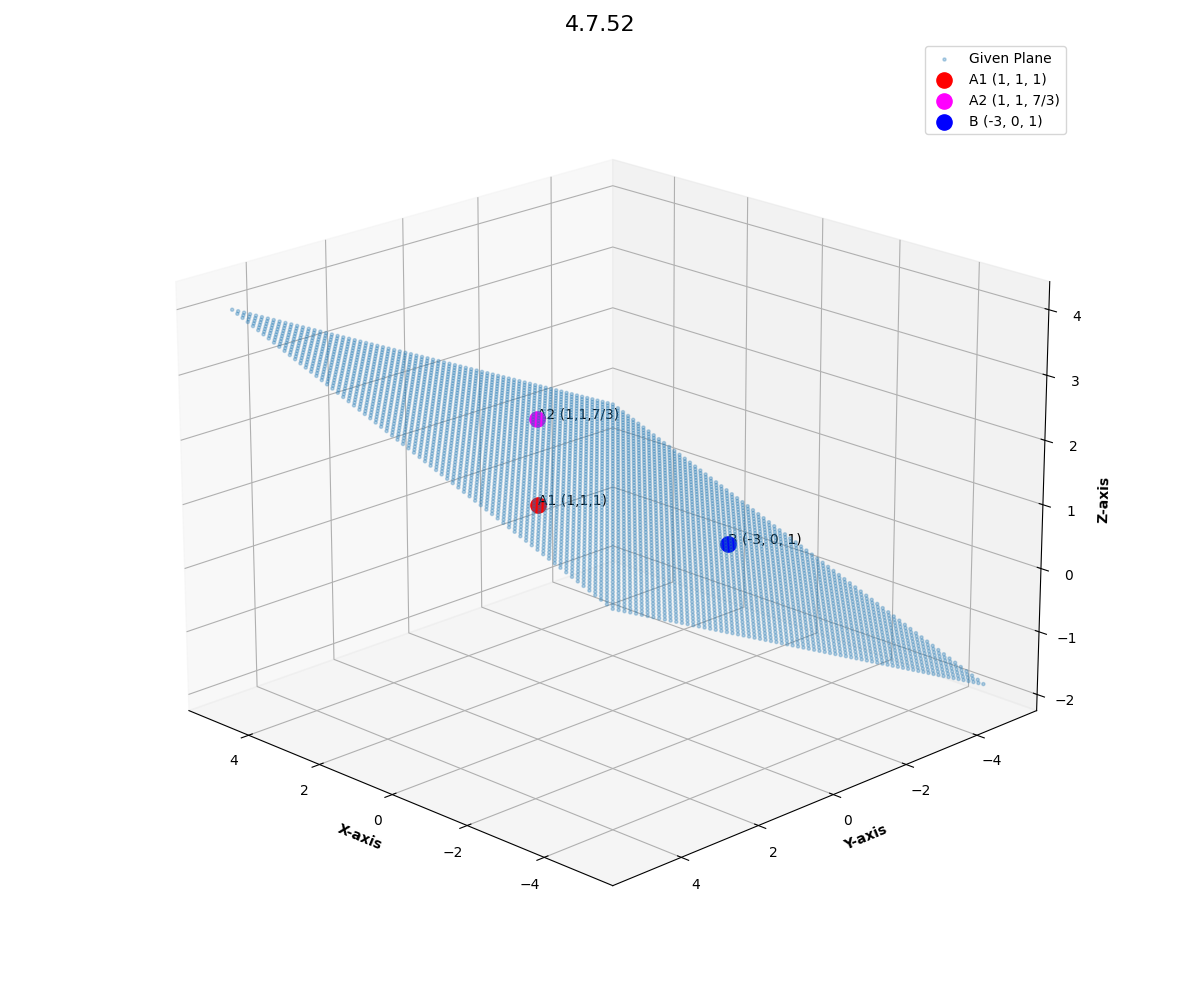
\includegraphics[width=0.8\columnwidth]{../figs/plot.png}
    \caption*{}
    \label{fig:plot}
\end{figure}
\end{frame}

\section{C Code}
\begin{frame}[fragile]{C code for generating points on plane}
\begin{lstlisting}[language=C]
 void generate_plane_points(
    // Output params
    double* x_coords, double* y_coords, double* z_coords,
    // Grid params
    double x_min, double x_max, int x_steps,
    double y_min, double y_max, int y_steps,
    // Plane stuff
    double n1, double n2, double n3, double c) {

    double x_step_val = (x_max - x_min) / (x_steps - 1);
    double y_step_val = (y_max - y_min) / (y_steps - 1);
    int index = 0;
\end{lstlisting}
\end{frame}
\begin{frame}[fragile]{C code for generating points on a plane}
\begin{lstlisting}[language=C]
    for (int i = 0; i < x_steps; i++) {
        for (int j = 0; j < y_steps; j++) {
            double current_x = x_min + i * x_step_val;
            double current_y = y_min + j * y_step_val;
            double current_z;
            // Vertical plane check
            if ((c < 1e-9)&&(c > -1e-9)) {
                current_z = 0.0;
            } else {
                current_z = (-n1 * current_x - n2 * current_y + c) / n3;
            }
            x_coords[index] = current_x;
            y_coords[index] = current_y;
            z_coords[index] = current_z;
            index++;
        }
    }
}
\end{lstlisting}
\end{frame}

\section{Python Code}
\subsection{Using shared objects}
\begin{frame}[fragile]{Python code for plotting using C}
\begin{lstlisting}[language=Python]
import ctypes
import numpy as np
import matplotlib.pyplot as plt

lib = ctypes.CDLL("./plane.so")
lib.generate_plane_points.argtypes = [
    ctypes.POINTER(ctypes.c_double),
    ctypes.POINTER(ctypes.c_double),
    ctypes.POINTER(ctypes.c_double),
    ctypes.c_double, ctypes.c_double, ctypes.c_int,
    ctypes.c_double, ctypes.c_double, ctypes.c_int,
    ctypes.c_double,
    ctypes.c_double,
    ctypes.c_double,
    ctypes.c_double,
]
lib.generate_plane_points.restype = None
\end{lstlisting}
\end{frame}
\begin{frame}[fragile]
 \begin{lstlisting}[language=Python]
A1 = np.array([1, 1, 1]).T
A2 = np.array([1, 1, 7 / 3]).T
B = np.array([-3, 0, 1]).T
n = np.array([3, 4, -12]).T
c = -13
x_steps, y_steps = 70, 70
total_points = x_steps * y_steps
x_plane = np.zeros(total_points, dtype=np.double)
y_plane = np.zeros(total_points, dtype=np.double)
z_plane = np.zeros(total_points, dtype=np.double)
lib.generate_plane_points(
    x_plane.ctypes.data_as(ctypes.POINTER(ctypes.c_double)),
    y_plane.ctypes.data_as(ctypes.POINTER(ctypes.c_double)),
    z_plane.ctypes.data_as(ctypes.POINTER(ctypes.c_double)),
    -5.0, 5.0, x_steps,
    -5.0, 5.0, y_steps,
    n[0], n[1], n[2],
    c,
)
 \end{lstlisting}
\end{frame}
\begin{frame}[fragile]
 \begin{lstlisting}[language=Python]
fig = plt.figure(figsize=(8, 6))
ax = fig.add_subplot(111, projection="3d")
t_values = np.linspace(0, 1, 100)
line_points_x, line_points_y, line_points_z = [], [], []
for t in t_values:
    result_arr = DoubleArray3()

    get_point(o, a, t, result_arr)

    line_points_x.append(result_arr[0])
    line_points_y.append(result_arr[1])
    line_points_z.append(result_arr[2])
ax.plot(
    line_points_x,
    line_points_y,
    line_points_z,
    color="red",
    label="a",
)
 \end{lstlisting}
\end{frame}
\begin{frame}[fragile]
 \begin{lstlisting}[language=Python]
ax.set_xlabel("X-axis", fontweight="bold")
ax.set_ylabel("Y-axis", fontweight="bold")
ax.set_zlabel("Z-axis", fontweight="bold")
ax.set_title("4.7.52", fontsize=16)
ax.view_init(elev=20, azim=135)
ax.legend()
plt.tight_layout()
plt.savefig("../figs/plot.png")
plt.show()
 \end{lstlisting}
\end{frame}

\subsection{Plot}
\begin{frame}{Plot}
 \begin{figure}[H]
    \centering
    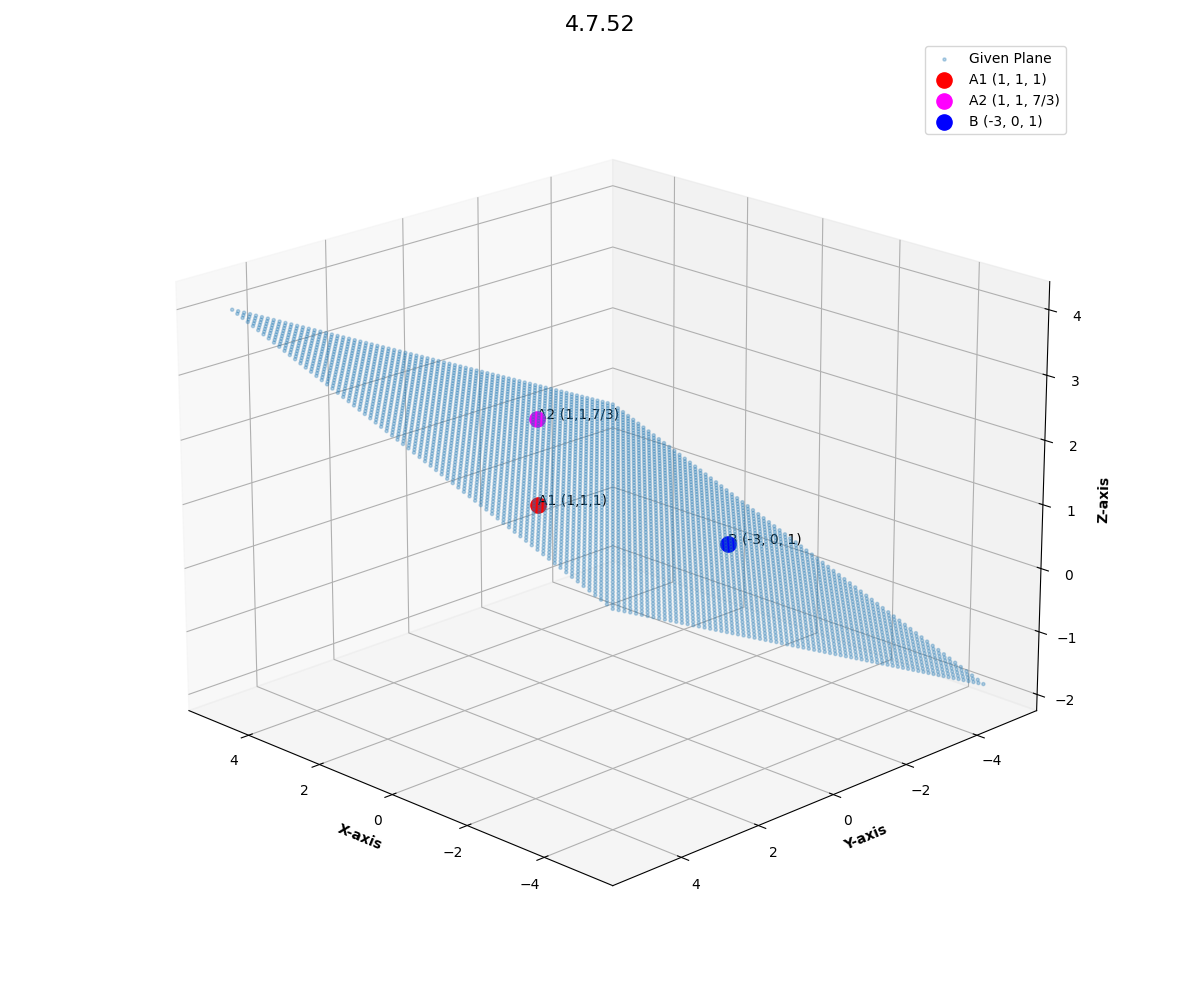
\includegraphics[width=0.8\columnwidth]{../figs/plot.png}
    \caption*{}
    \label{fig:plot}
\end{figure}
\end{frame}
\subsection{In pure Python}
\begin{frame}[fragile]{Pure Python code}
 \begin{lstlisting}[language=Python]
import numpy as np
import matplotlib.pyplot as plt
from mpl_toolkits.mplot3d import Axes3D

n = np.array([3, 4, -12]).T
d = -13
a = np.array([-3, 0, 1]).T
b = np.array([1, 1, 1]).T
c = np.array([1, 1, 7 / 3]).T

fig = plt.figure(figsize=(8, 8))
ax = fig.add_subplot(111, projection="3d")


x, y = np.meshgrid(range(10), range(10))
z = -(n[0] * x + n[1] * y - d) / n[2]
ax.plot_surface(x, y, z, alpha=0.7, color="gray")

 \end{lstlisting}
\end{frame}
\begin{frame}[fragile]{Pure Python code}
 \begin{lstlisting}[language=Python]
ax.scatter(a[0], a[1], a[2], color="red", label="a")
ax.scatter(b[0], b[1], b[2], color="blue", label="b")
ax.scatter(c[0], c[1], c[2], color="green", label="c")
ax.text(a[0], a[1], a[2], "Given Point")
ax.text(b[0], b[1], b[2], "Point 1")
ax.text(c[0], c[1], c[2], "Point 2")
ax.set_xlabel("X-axis")
ax.set_ylabel("Y-axis")
ax.set_zlabel("Z-axis")
ax.set_title("2.9.6")
ax.set_xlim([-5, 10])
ax.set_ylim([-5, 10])
ax.set_zlim([-5, 10])
ax.legend()
ax.grid(True)
plt.savefig("../figs/python.png")
plt.show()
 \end{lstlisting}
\end{frame}
\subsection{Plot}
\begin{frame}{Plot}
 \begin{figure}[H]
    \centering
    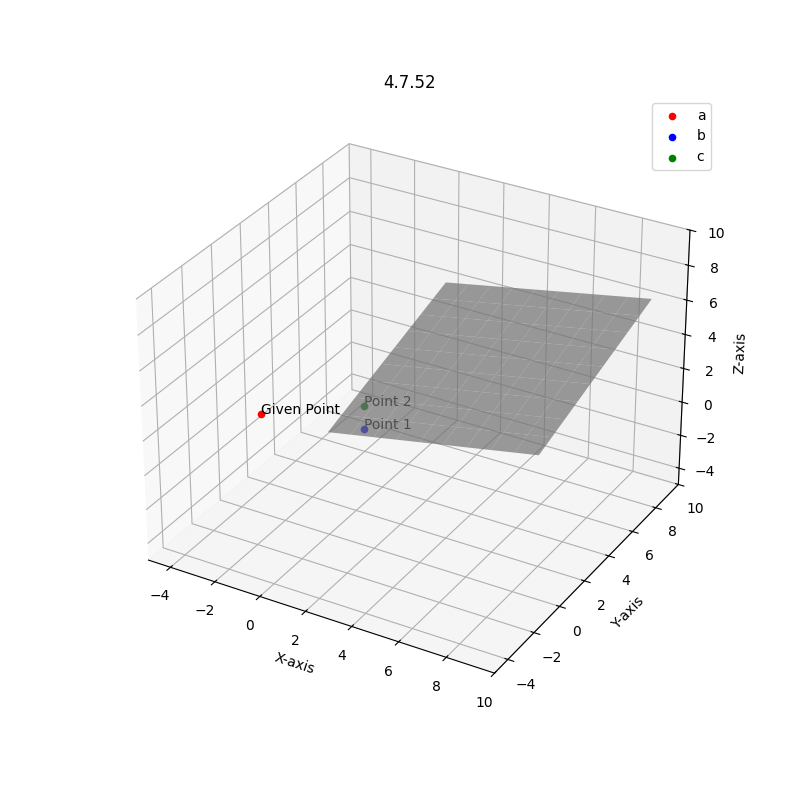
\includegraphics[width=0.75\columnwidth]{../figs/python.png}
    \caption*{}
    \label{fig:plot}
\end{figure}
\end{frame}
\end{document}
